% DIAGNOSTIC_ONLY; synthetic cloud, incomplete exact-source convergence evidence.
\begin{figure*}[t]
\centering
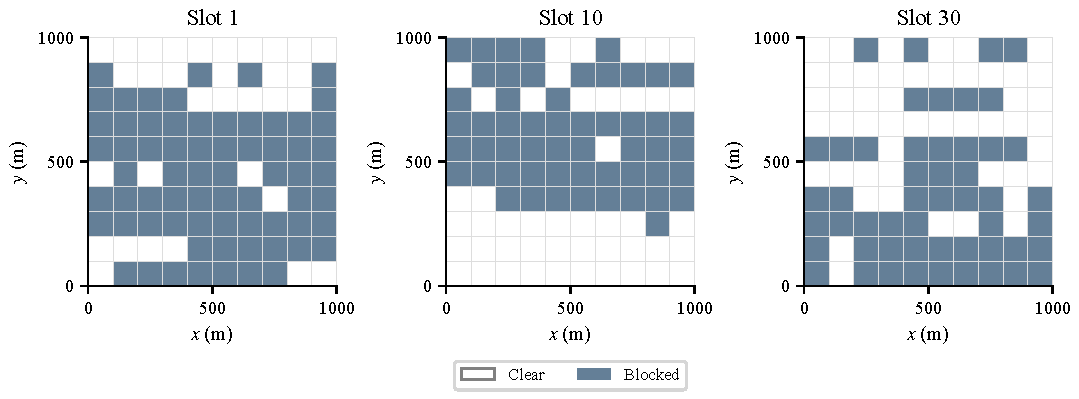
\includegraphics[width=\textwidth]{fig1_cloud_realizations.pdf}
\caption{Independent-slot binary cloud fields at slots 1, 10, and 30 of mission 0, zero-threshold mode. White cells are clear and shaded cells blocked. The row-major index covariance is not distance-isotropic. Primary HAP projection is (500,500) m. Results are diagnostic and conditional on incomplete source-convergence evidence; no QKD security certification is claimed.}
\label{fig:fig1_cloud_realizations}
\end{figure*}

\begin{figure*}[t]
\centering
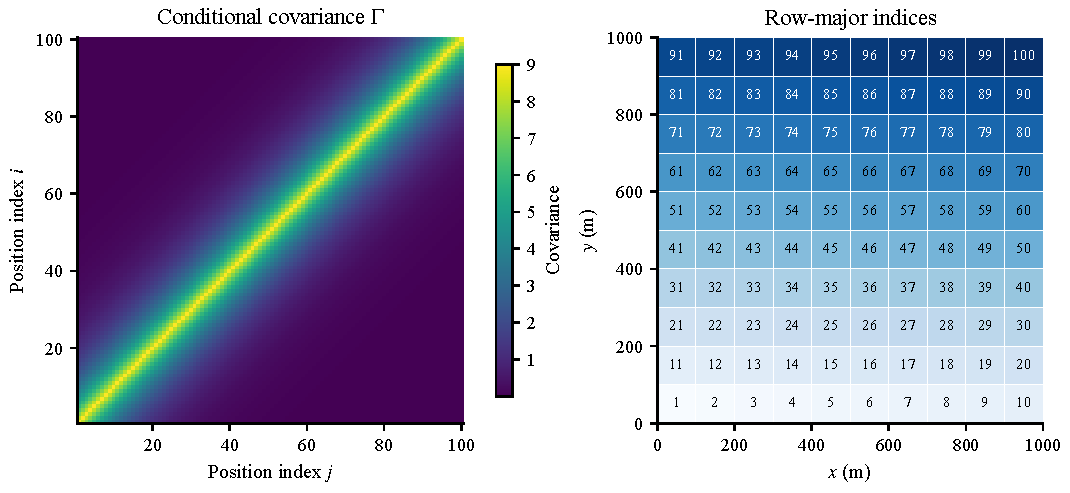
\includegraphics[width=\textwidth]{fig2_cloud_covariance.pdf}
\caption{Exact conditional covariance $\Gamma_{ij}=9(0.9)^{|i-j|}$ and row-major mapping of the 100 candidate positions. Horizontal and vertical nearest neighbors have conditional Gaussian correlations $0.9$ and $0.9^{10}$, despite equal grid spacing. Primary HAP projection is (500,500) m. Results are diagnostic and conditional on incomplete source-convergence evidence; no QKD security certification is claimed.}
\label{fig:fig2_cloud_covariance}
\end{figure*}

\begin{figure*}[t]
\centering
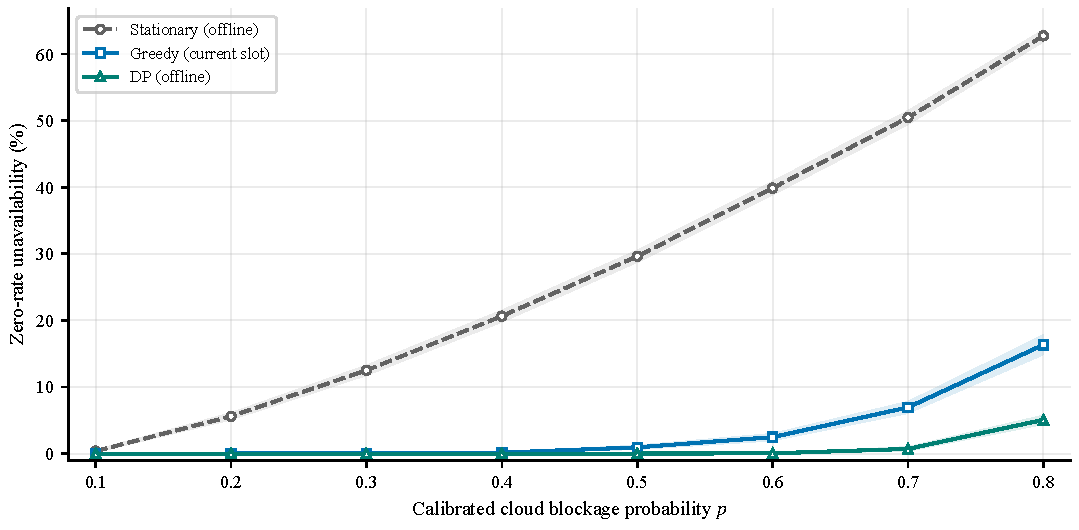
\includegraphics[width=\textwidth]{fig3_unavailability_vs_p.pdf}
\caption{Zero-rate unavailability versus calibrated blockage probability for optimal Stationary, current-slot Greedy, and offline DP. Bands are pointwise 95% Student-t intervals across 100 paired missions; observed zero outages do not establish zero population risk. Primary HAP projection is (500,500) m. Results are diagnostic and conditional on incomplete source-convergence evidence; no QKD security certification is claimed.}
\label{fig:fig3_unavailability_vs_p}
\end{figure*}

\begin{figure*}[t]
\centering
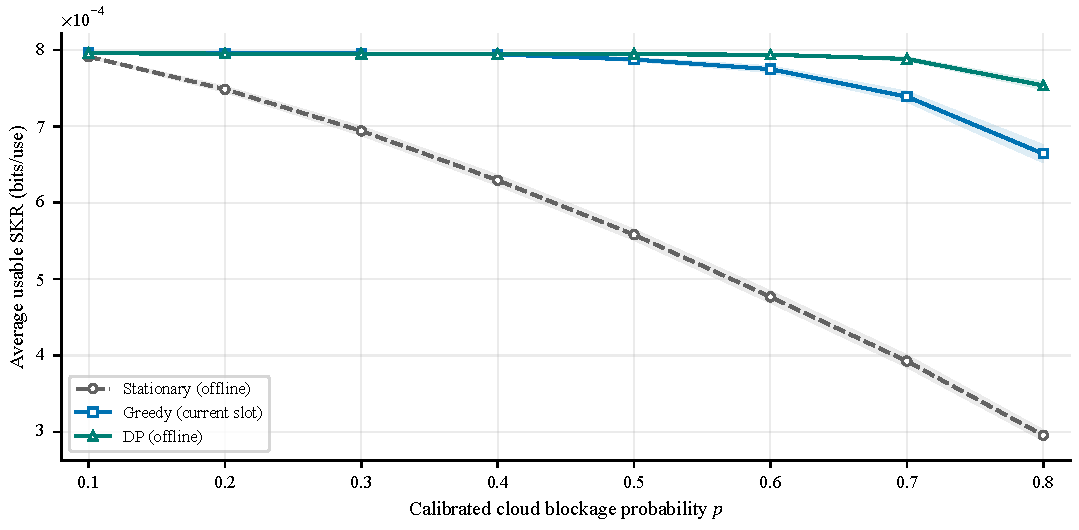
\includegraphics[width=\textwidth]{fig4_usable_skr_vs_p.pdf}
\caption{Average usable SKR versus calibrated blockage probability for the three positioning algorithms, using the same position-dependent Optimized MB clear-sky map and cloud states. Bands are pointwise 95% mission-mean intervals. Primary HAP projection is (500,500) m. Results are diagnostic and conditional on incomplete source-convergence evidence; no QKD security certification is claimed.}
\label{fig:fig4_usable_skr_vs_p}
\end{figure*}

\begin{figure*}[t]
\centering
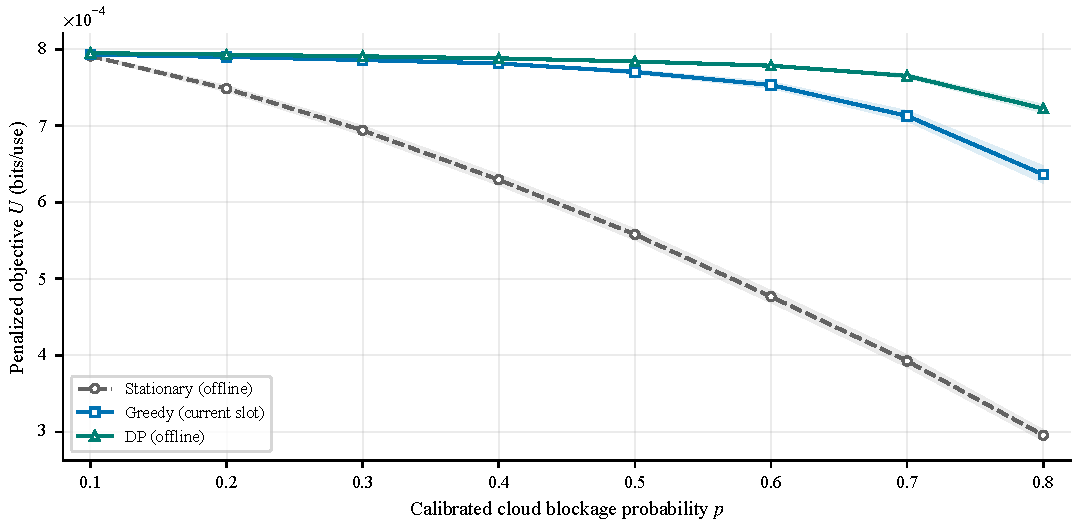
\includegraphics[width=\textwidth]{fig5_objective_vs_p.pdf}
\caption{Penalized objective $U=\bar S-\lambda D/D_{\rm ref}$ versus calibrated blockage probability at $\lambda=9.468026677248516\times10^{-6}$ bits/use. DP and optimal Stationary use offline mission knowledge; Greedy does not. Primary HAP projection is (500,500) m. Results are diagnostic and conditional on incomplete source-convergence evidence; no QKD security certification is claimed.}
\label{fig:fig5_objective_vs_p}
\end{figure*}

\begin{figure*}[t]
\centering
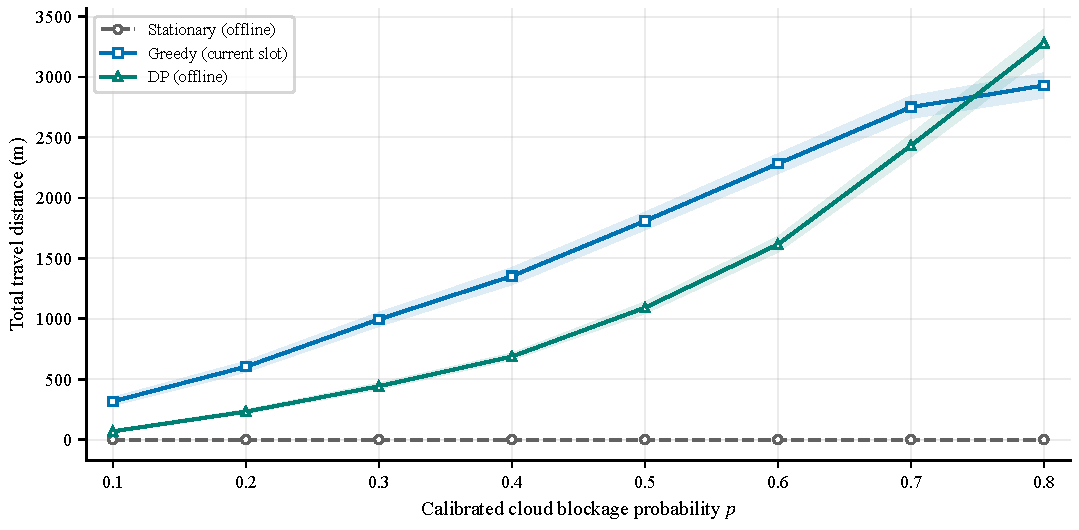
\includegraphics[width=\textwidth]{fig6_distance_vs_p.pdf}
\caption{Total UAV travel distance versus calibrated blockage probability. Stationary travel is zero. DP maximizes the penalized objective and is not required to minimize distance individually. Shading indicates pointwise 95% mission-mean intervals. Primary HAP projection is (500,500) m. Results are diagnostic and conditional on incomplete source-convergence evidence; no QKD security certification is claimed.}
\label{fig:fig6_distance_vs_p}
\end{figure*}

\begin{figure*}[t]
\centering
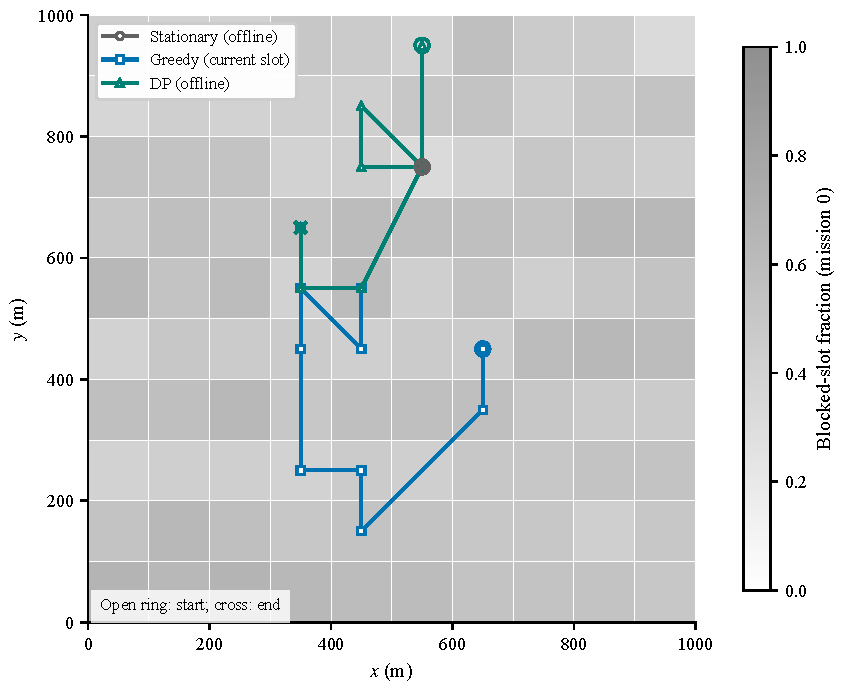
\includegraphics[width=\textwidth]{fig7_representative_trajectories.pdf}
\caption{Paired trajectories for mission 0 in zero-threshold mode at the reference mobility penalty. The background shows the fraction of blocked slots over the mission, not a fixed cloud. Open rings and crosses indicate initial and final positions. DP and optimal Stationary are offline benchmarks; Greedy uses only current-slot states. Primary HAP projection is (500,500) m. Results are diagnostic and conditional on incomplete source-convergence evidence; no QKD security certification is claimed.}
\label{fig:fig7_representative_trajectories}
\end{figure*}

\begin{figure*}[t]
\centering
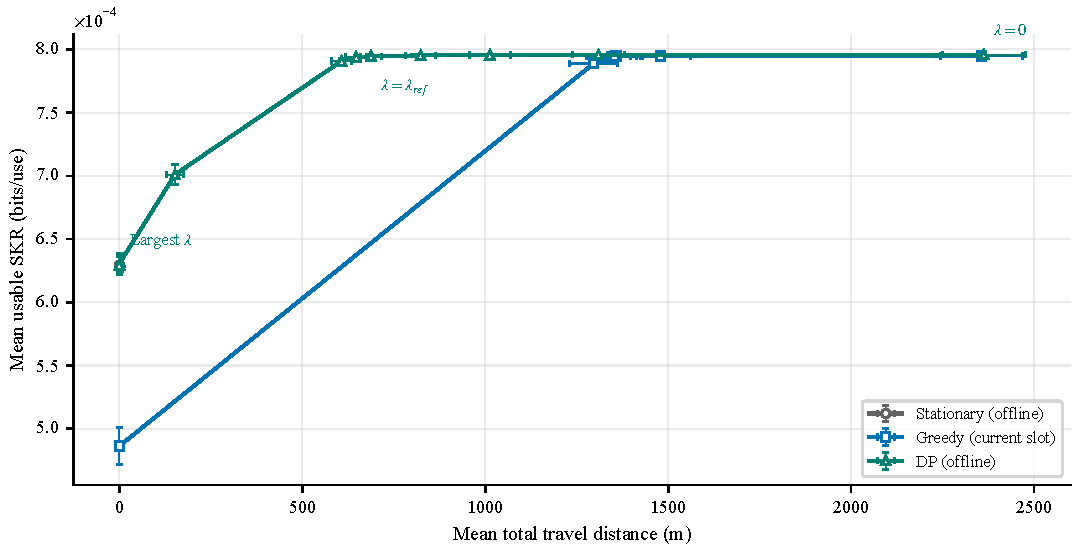
\includegraphics[width=\textwidth]{fig8_mobility_penalty_tradeoff.pdf}
\caption{Mean usable-rate versus travel-distance tradeoff at calibrated $p=0.4$ for the ten historical mobility penalties, including zero and $\lambda_{\rm ref}$. Error bars are pointwise 95% intervals over the same 100 paired missions. Lines only join the tested penalty settings. Primary HAP projection is (500,500) m. Results are diagnostic and conditional on incomplete source-convergence evidence; no QKD security certification is claimed.}
\label{fig:fig8_mobility_penalty_tradeoff}
\end{figure*}
